\chapter{Konzeption}\label{chapter:concept}
%%%%%%%%%%%%%%%%%%%%%%%%%%%%%%%%%%%%%%%%%%%%%%%%%%%%%%%%%%%%

\imiscomment{Grobkonzeption der Arbeit}

\imiscomment{Keine Codedarstellung, allenfalls Pseudocode}

\imiscomment{Struktur dieses Kapitel kann je nach Problemstellung unterschiedlich gestaltet werden}

%%%%%%%%%%%%%%%%%%%%%%%%%%%%%%%%%%%%%%%%%%%%%%%%%%%%%%%%%%%%
\section{Systemarchitektur}\label{sec:architecture}
%%%%%%%%%%%%%%%%%%%%%%%%%%%%%%%%%%%%%%%%%%%%%%%%%%%%%%%%%%%%

\imiscomment{Struktur des Gesamtsystems mit seinen Subsystemen}

% this is an example for using TikZ:
\begin{figure}[htb]
  \begin{center}
    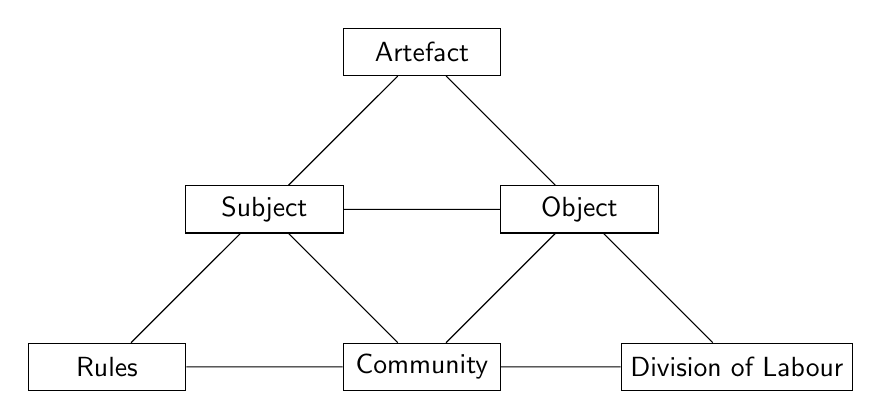
\begin{tikzpicture}[minimum width=2cm,minimum height=0.6cm]
      {\sffamily
        \node (artefact)      at (2,0)  [draw] {Artefact};
        \node (subject)       at (0,-2) [draw] {Subject};
        \node (object)        at (4,-2) [draw] {Object};
        \node (rules)         at (-2,-4) [draw] {Rules};
        \node (community)     at (2,-4) [draw] {Community};
        \node (dol)           at (6,-4) [draw] {Division of Labour};

        \draw (artefact) -- (subject) -- (object) -- (artefact);
        \draw (subject) -- (rules) -- (community) -- (dol) -- (object) -- (community) -- (subject);
      }
    \end{tikzpicture}
  \end{center}
  \caption{{Cultural Historical Activity Theory: Expanded triangle, incorporating the community and other mediators.}}
  \label{fig:chat}
\end{figure}

%%%%%%%%%%%%%%%%%%%%%%%%%%%%%%%%%%%%%%%%%%%%%%%%%%%%%%%%%%%%
\subsection{Konzeption von Modul 1}\label{subsec:concept_module_1}
%%%%%%%%%%%%%%%%%%%%%%%%%%%%%%%%%%%%%%%%%%%%%%%%%%%%%%%%%%%%

\imiscomment{Grobkonzeption eines einzelnen Moduls}

%%%%%%%%%%%%%%%%%%%%%%%%%%%%%%%%%%%%%%%%%%%%%%%%%%%%%%%%%%%%
\subsection{Konzeption von Modul 2}\label{subsec:concept_module_2}
%%%%%%%%%%%%%%%%%%%%%%%%%%%%%%%%%%%%%%%%%%%%%%%%%%%%%%%%%%%%